\chapter{物理的背景}
\section{分子動力学法}
分子動力学法は運動方程式を解く事によって,粒子の振る舞いを解析する手法である\cite{MD}.ニュートンの運動方程式はエネルギー保存則を満たすため,エネルギーが保存される集団において用いられる.
\subsection{Verlet法}
Verlet法は分子動力学法における粒子の座標を逐次的に求める方法であり,式(\ref{eq:verlet})のように表される.
\begin{eqnarray}
\label{eq:verlet}
r(t+h)=2r(t)-r(t-h)+\frac{h^2}{m}f(t)
\end{eqnarray}
ここで,$r(t)$は時刻$t$における粒子の座標,$f(t)$は時刻$t$における粒子に加わっている力,$h$は微小時間,$m$は粒子の質量を表している.
式(\ref{eq:verlet})は,時刻$t$における粒子の座標,時刻$t-h$における粒子の座標,時刻$t$における粒子に加わっている力,粒子の質量の4つの要素から,時刻$t+h$における粒子の座標が求まることを表している.
粒子に加わっている力を常に決定することができれば,Verlet法を継続的に用いることが可能であり,逐次的に粒子の座標を決定し続けることができる.
また,粒子を動かすために速度が必要そうだが,この手法では速度を必要としないという特徴がある.この手法はニュートンの運動方程式から導出されるため,エネルギーが保存される系で有効である.


\subsection{導出}
時刻$t+h$における粒子の座標$r(t+h)$にテイラー展開を行うと式(\ref{eq:verlet2})ができる.

\begin{eqnarray}
\label{eq:verlet2}
r(t+h)=r(t)+h\frac{dr(t)}{dt}+\frac{h^2}{2!}\frac{d^2r(t)}{dt^2}+\frac{h^3}{3!}\frac{d^3r(t)}{dt^3}+...
\end{eqnarray}

$h$は微小時間のため$h^3$以上の項を無視すると
\begin{eqnarray}
\label{eq:verlet5}
r(t+h)=r(t)+h\frac{dr(t)}{dt}+\frac{h^2}{2!}\frac{d^2r(t)}{dt^2}
\end{eqnarray}

$h$を$-h$に置き換えると
\begin{eqnarray}
\label{eq:verlet6}
r(t-h)=r(t)-h\frac{dr(t)}{dt}+\frac{h^2}{2!}\frac{d^2r(t)}{dt^2}
\end{eqnarray}

式(\ref{eq:verlet5})と式(\ref{eq:verlet6})を足し合わせ$r(t+h)$について移項させると式(\ref{eq:verlet3})ができる.

\begin{eqnarray}
\label{eq:verlet3}
r(t+h)=2r(t)-r(t-h)-h^2\frac{d^2r(t)}{dt^2}
\end{eqnarray}

ここでニュートンの運動方程式について考える.$v(t)$を時刻$t$の速度,$r(t)$を時刻$t$の位置とすると式(\ref{eq:newton})ができる.
\begin{eqnarray}
\label{eq:newton}
v(t)=\frac{dr(t)}{dt}
\end{eqnarray}
また,式(\ref{eq:newton})より時刻$t$における加速度$a(t)$は
\begin{eqnarray}
a(t)=\frac{d^2r(t)}{dt^2}
\end{eqnarray}
ここで$f(t)$を時刻$t$に作用する力,$m$を質量とするとニュートンの運動方程式は式(\ref{eq:newton2})となる.
\begin{eqnarray}
\label{eq:newton2}
f(t)=m\frac{d^2r(t)}{dt^2}
\end{eqnarray}
移項させると
\begin{eqnarray}
\label{eq:newton4}
\frac{f(t)}{m}=\frac{d^2r(t)}{dt^2}
\end{eqnarray}

式(\ref{eq:newton4})を式(\ref{eq:verlet3})にを代入すると式(\ref{eq:newton3})となりVerlet法が導出される.
\begin{eqnarray}
\label{eq:newton3}
r(t+h)=2r(t)-r(t-h)+\frac{h^2}{m}f(t)
\end{eqnarray}


\section{Lennard-Jonesポテンシャル}
Lennard-Jonesポテンシャルとは2体間での相互作用ポテンシャルエネルギーを経験則的に表したモデルである\cite{akahon}.$ψ$をポテンシャルエネルギー,$R$を原子間距離,$A$,$B$は任意の定数とすると式(\ref{eq:lennard})のように表される.
\begin{eqnarray}
\label{eq:lennard}
\psi(R)=A\bigg(\frac{1}{R}\bigg)^{12}+B\bigg(\frac{1}{R}\bigg)^6
\end{eqnarray}
式(\ref{eq:lennard})は縦軸をポテンシャルエネルギー,横軸を粒子間距離とすると図\ref{fig:lennard}のような概形になる.


ポテンシャルエネルギーの理解には,安定した状態からずれるとエネルギーが生じるという考え方が適切である.
図\ref{fig:lennard}では極小点が平衡原子間距離であり,双方の粒子が安定した状態であると言える.
原子間距離が安定状態より近くなれば,急激にエネルギーが上がる.これは近づくことで原子同士の影響力が増大するからである.
逆に,安定状態より遠くなると,エネルギーは緩やかに上がっていき,ある高さで上昇が止まる.これは原子同士の影響力が減少するからである.
これに加えて,原子に作用する力について考えていく.ポテンシャルエネルギーを距離で微分することにより作用する力が求まる
.図\ref{fig:lennard}の傾きに注目すると,
平衡原子間距離は極小点であり傾きは0のため力が作用しない.
また,距離が近くなれば傾きは急激に負の値をとり斥力が生まれる.逆に,遠くなれば傾きは正の値をとり引力が生まれるが,傾きが徐々に0に近づくため力が弱まっていく.このように図\ref{fig:lennard}のような概形のポテンシャルエネルギーは,バネのような振る舞いをすることがわかる.
\begin{figure}[htbp]
 \begin{center}
  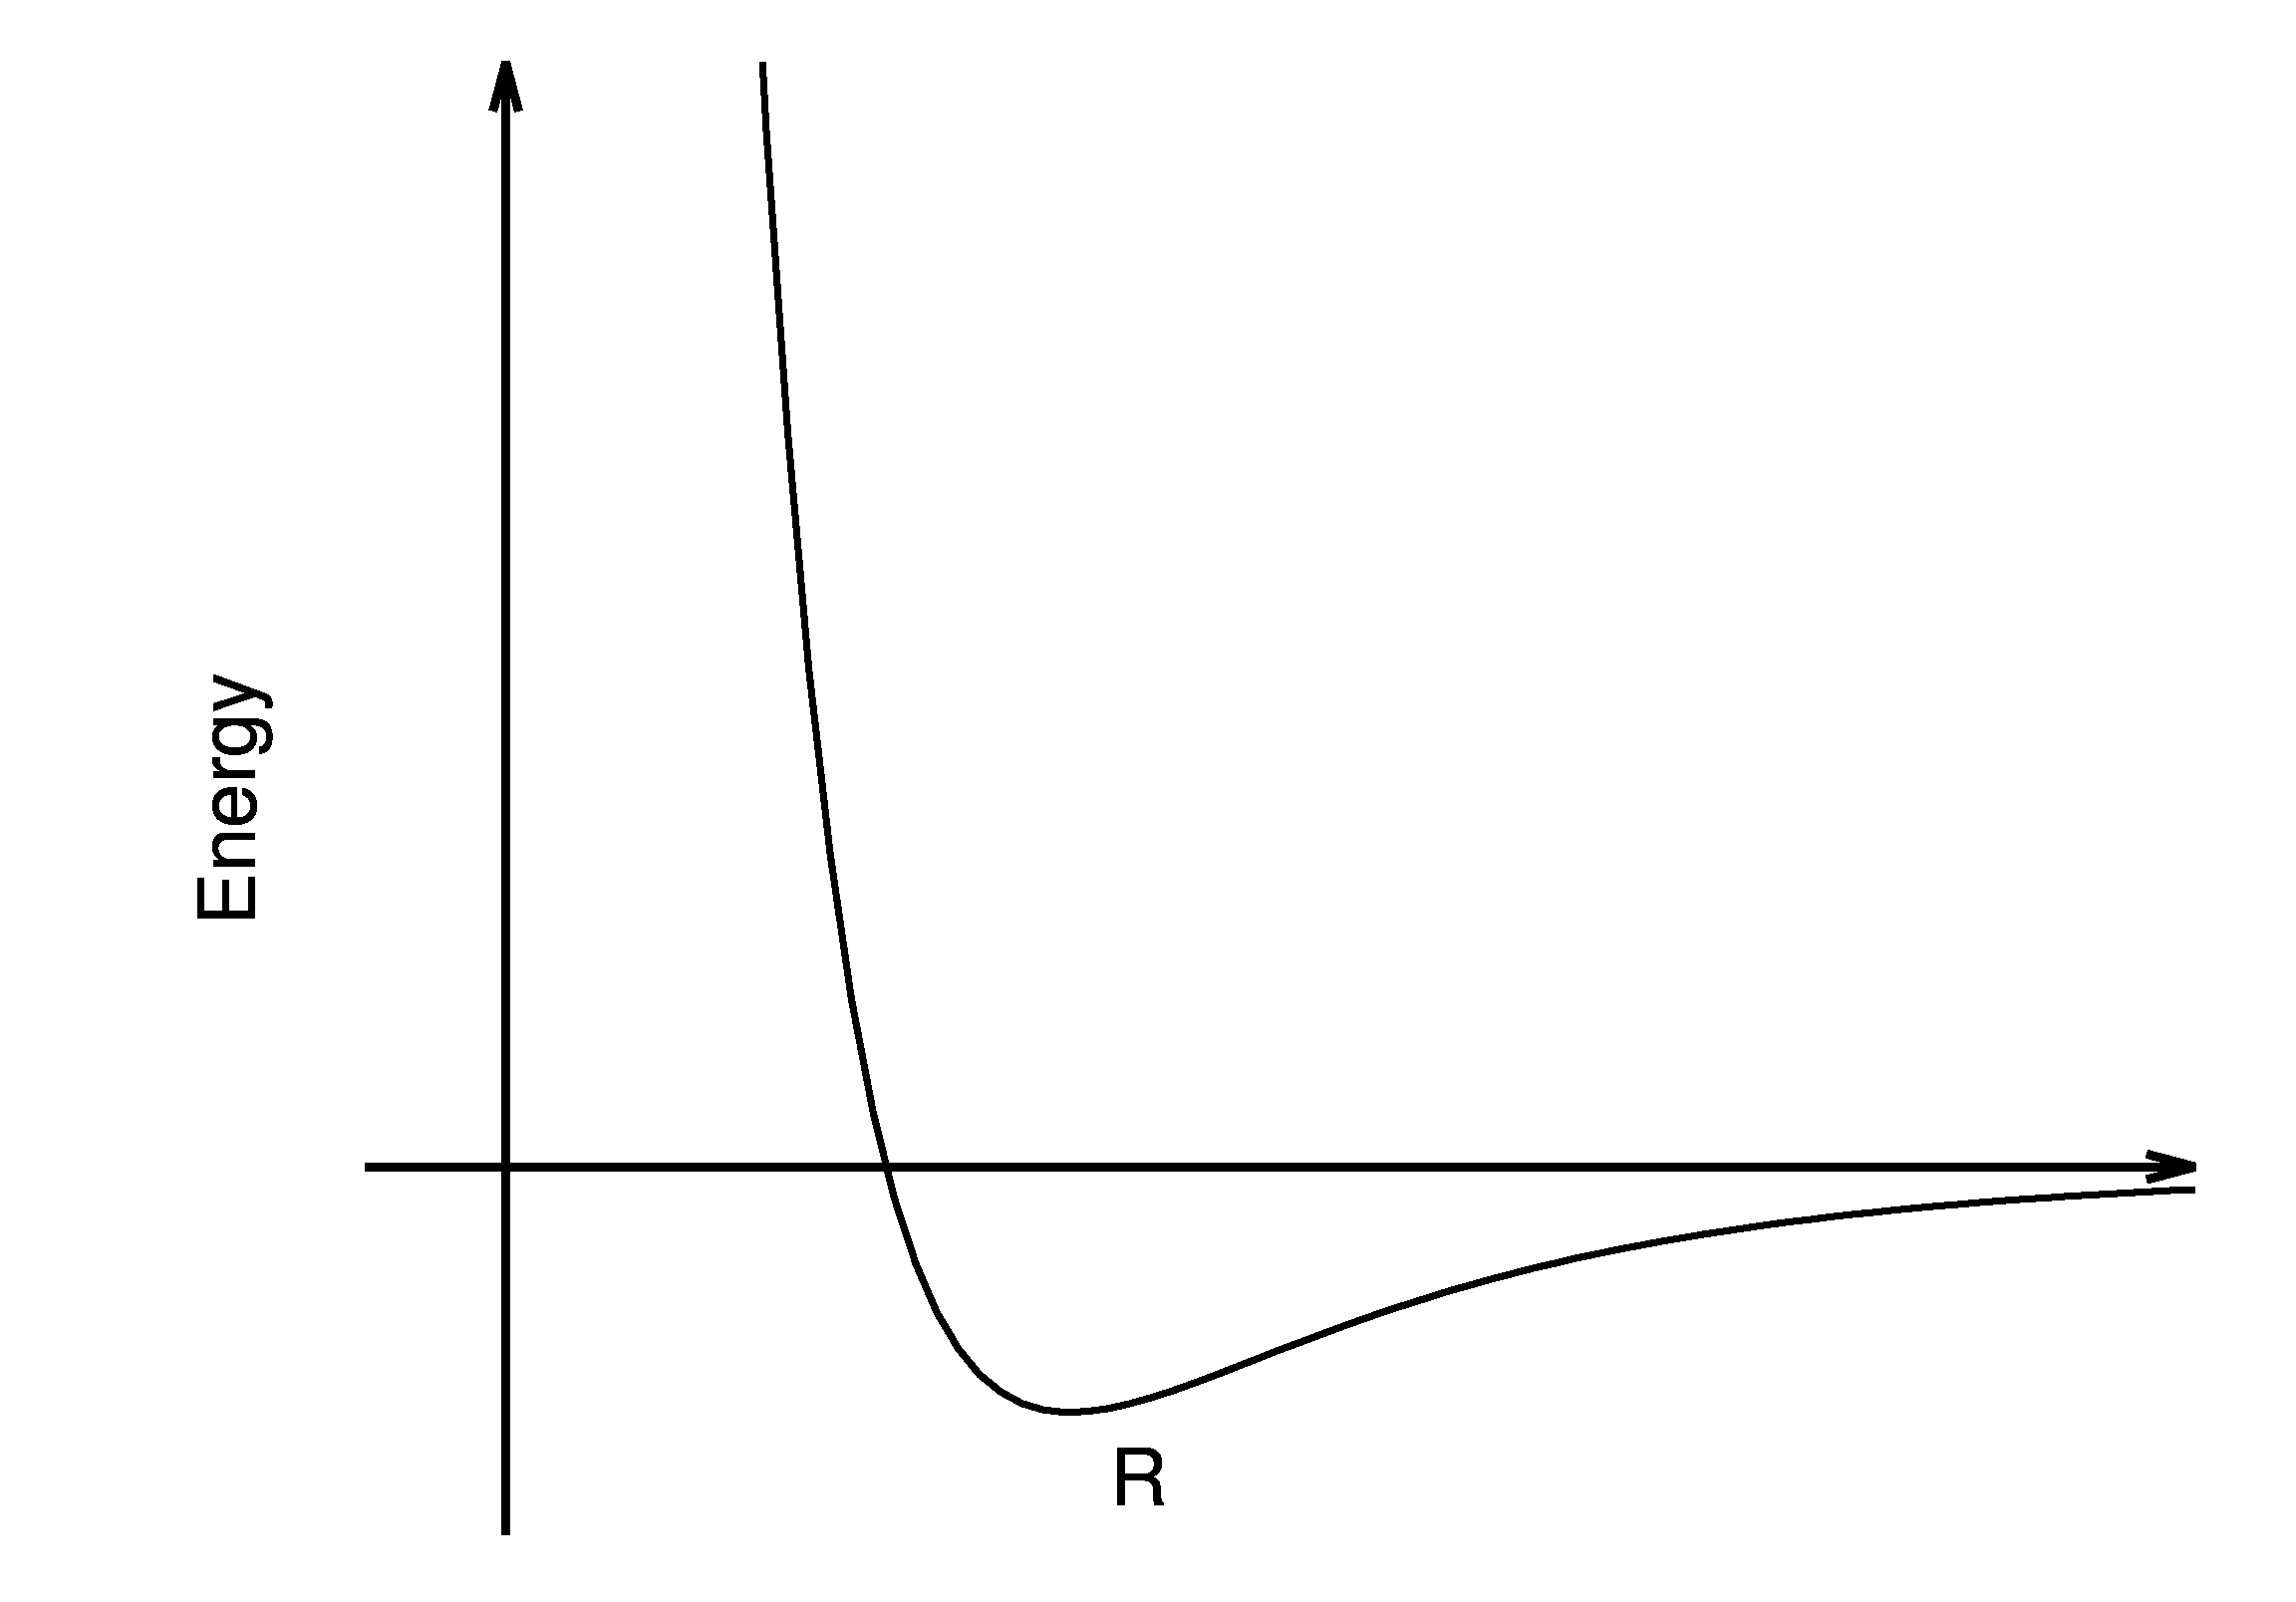
\includegraphics[width=150mm]{../intro/lennard.png}
 \end{center}
 \caption{Lennard-Jonesポテンシャル.}
 \label{fig:lennard}
\end{figure}